\subsection{Interacting With User threads}
\textbf{Definition}
A user thread is a thread that is not created by OpenMP implementation. A user thread 
could become an OpenMP initial thread. 

The most common example of user threads are POSIX Threads, 
usually referred to as Pthreads with implementation available on most Unix-like 
POSIX-compliant systems. There are also implementations of other thread libraries, 
for example, Windows Native threads and language based threading support such as 
Java threads or others (e.g. qthreads). 

Figure~\ref{fig:pthread-omp} shows an example of having three user 
threads (two PThreads and one thread of the main program) in an OpenMP program. 
The two three threads execute in parallel after the two PThreads are created. 
Each thread calls a function that will enter into
OpenMP threading parallelism. So they all become OpenMP initial threads. How the 
user threads (PThreads in this example) interact with the OpenMP threading mechanisms
in the runtime is up to the implementation. They may share the same OpenMP runtime
instance or each has its own OpenMP runtime instance. 

\begin{figure}[t]
\centering
  \fbox{
 % \lstset{basicstyle=\ttfamily\scriptsize,language=c}
  \lstset{basicstyle=\ttfamily\scriptsize,language=c,numbers=left, %,frame=single,
  deletekeywords={int,if,else,while},
  morekeywords={pragma,omp,target,device,map,
  tofrom,to,from,alloc,parallel,shared,reduction,data,collapse,
  private,dist_iteration,match_range,halo,exchange},
  numbersep=12pt,numberstyle=\color{red}}
  \lstinputlisting{pthread-omp.c}

}
\caption{Three user threads (two Pthreads and one main thread) with OpenMP}
  \label{fig:pthread-omp}
\end{figure}

\subsection{Impacts and Discussions}
A user thread in a program adds additional level(s) in the overall ``threading''
hierarchy of a program. Those additional levels could be on top of OpenMP threading 
mechanism when a user thread becomes an OpenMP initial thread that creates OpenMP thread
parallelism, or beneath the OpenMP threading mechanism when an OpenMP thread spawns 
a user thread, or the the mix of both. In the example from Figure~\ref{fig:pthread-omp}, 
one can view this in a two-level threading parallelism: the top level user thread 
parallelism and the bottom level OpenMP threading parallelism.

These additional levels of threading increase the complexity of a program, both for 
users in the aspect of reasoning the parallel and synchronization behavior of a program, 
and also for the implementation and runtime system in terms of resource management and 
interactions. Adding to the complexity is the facts that a user thread may be created 
through a call to a library function whose paralelism (OpenMP) behavior is not known to 
the callee. Typical issues for example: 
\begin{itemize}
\item Does each user thread use the same OpenMP runtime libraries or not? 
	If not using the same library, how to handle symbol name 
	conflicts of two more different OpenMP runtime libraries. 
\item For user threads that use the same OpenMP runtime library, does the user threads each create its own runtime instance or they share one?
\item For user threads each of which has its own runtime instance (from the same or 
	different runtime library), how to coordinate the resource management among those
	runtime instances to address such issues as oversubscriptions and the affinity
	between user threads?
\end{itemize}

It is important to note that approaches to address those issues are very implementation
dependent, requiring protocol and agreement in the runtime behavior and/or interfaces 
of different OpenMP implementations. It may not be realistic to solve some of the issue
from the language standard, and should be left to users to deal with them. In this
aspect, we still hope this report could provide userful information and practices 
for users. 



\subsection{Interacting With Other Parallel Systems or Libraries}
It is now very common that an application uses multiple parallel libraries at the same time, which could be developed 
using OpenMP, TBB, Cilkplus, C++11, and other parallel libraries. 

\begin{figure}[h!]
  \centering
      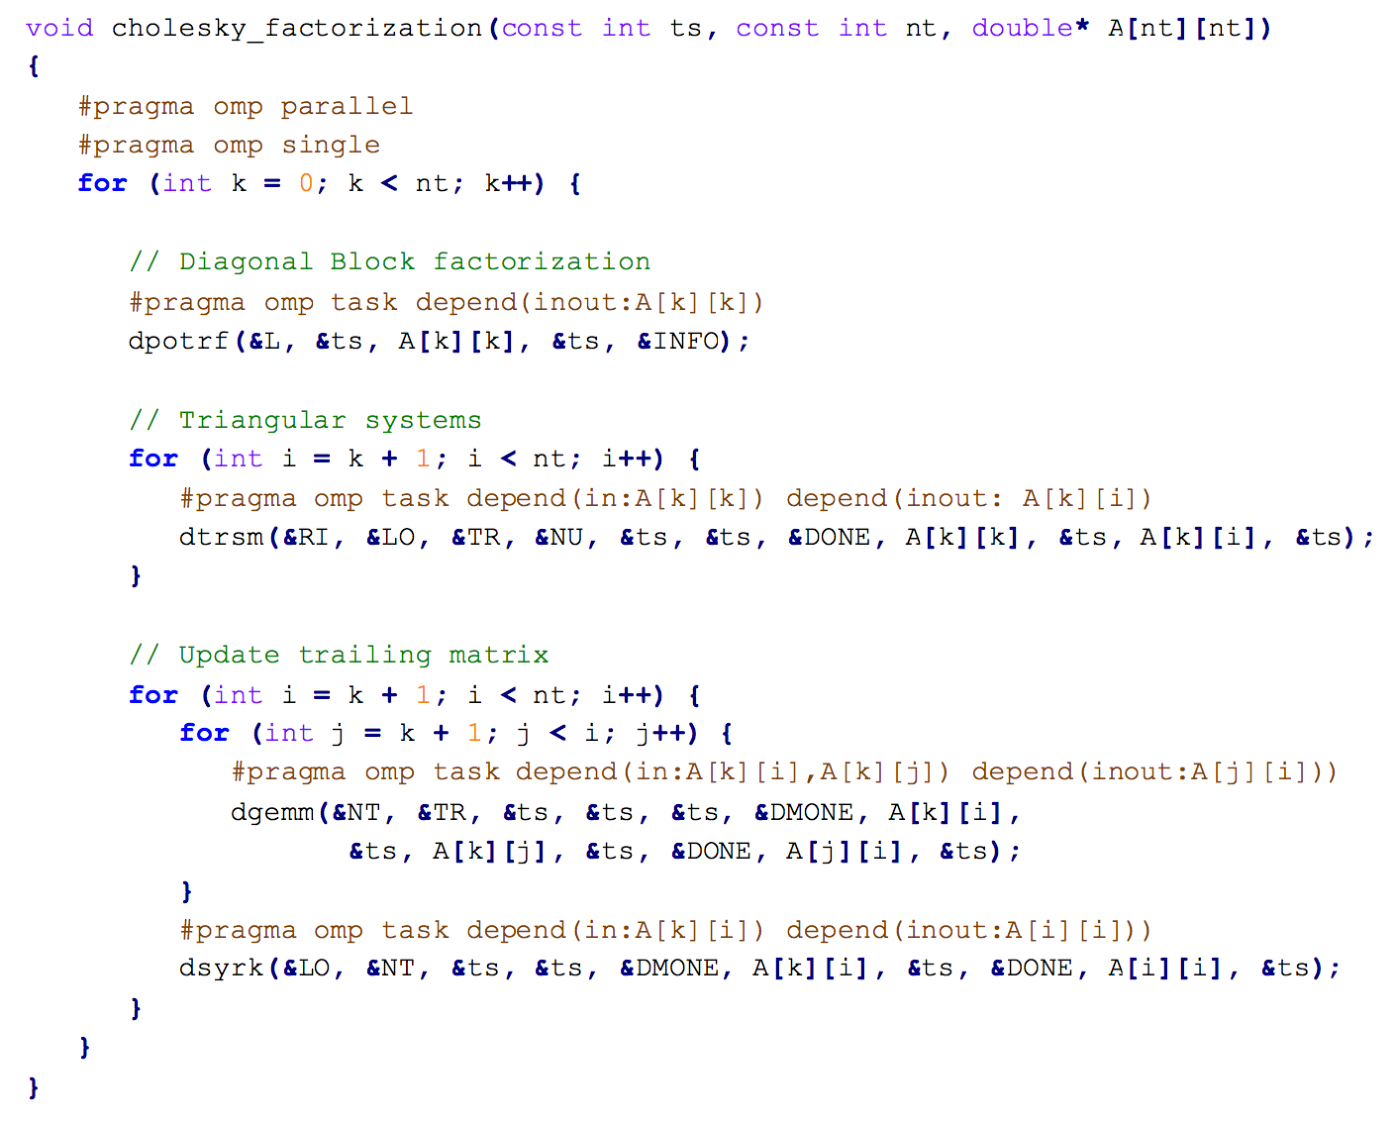
\includegraphics[width=0.85\textwidth]{images/cholesky}
      \caption{The Mixed Use of OpenMP Tasking and Intel MKL Library for Cholesky Factorization~\cite{intertwine}}
 \label{fig:cholesky}
\end{figure}


\subsection{Interoperability with inter-node programming model, e.g. MPI}
Hybrid parallel programming in the form of internode+intranode, e.g. MPI+X model are widely used for 
for high-performance computing. This approach reflects the two-level hierarchy of parallelism in current HPC systems, 
in which a high-speed interconnect
joins many highly parallel nodes.
Interoperability between inter-node programming model such as MPI and OpenMP 
systems has long been a productivity and composability goal within
the parallel programming community. We however still have not agreed on a standard solution from either of the two communities. 




\subsection{Oversubscription}
Oversubscription happens when resources are claimed and held than what is needed.
A program may request more OpenMP threads than the total amount of hardware
threads available when entering a parallel region, which causes excessive competition 
among OpenMP threads for hardware threads and increases runtime overhead. 
When program execution enters into sequential stage after exiting a parallel region, 
those native threads that support the OpenMP threads in the parallel region may still 
alive in the background consuming CPU cycles. This 
will make those hardware threads unavailable to others. 
Oversubscription impact the performance of an applications and the system, 
but should not introduce correctness issue to a program. 

%A typical OpenMP runtime creates a pool of native threads who will execute OpenMP
% parallel regions and/or tasks. 

The two scenarios we mentioned above are the two kinds of oversubscription we should try to avoid:
{\bf 1) Active oversubscription}: Claiming or requesting more threads than 
what are available by the system.
{\bf 2) Passive oversubscription}: Thread resources are not released 
after parallel execution. Holding hardware threads after parallel execution may not 
always hurt the performance overall, e.g. it will improve the start-up performance of the 
upcoming parallel region. In this category, we are concerning those situations that 
actually impact the performance negatively.




	\REM{
\subsection{Use Cases}
We have identified several use cases of OpenMP interoperating with itself and other parallel programming models. 
\subsubsection{OpenMP with native threads}
\subsubsection{OpenMP with TBB/MKL}
\subsubsection{OpenMP with parallel scientific library, such as MKL}
\subsubsection{Linking libraries and objects built with different OpenMP compilers}
\subsubsection{OpenMP with inter-node model, e.g. MPI}

\subsection{Issues and Possible Solutions}
\subsubsection{Active Oversubscription}
\subsubsection{Passive Oversubscription}
\subsubsection{Interop across contention group}
}

There are still some challenges in terms of OpenMP interoperability. 
OpenMP threads that are created by the parallel construct cannot interact with external systems. 
In other words, we are trying to enable the interoperability through flexible communication between OpenMP threads and user threads. 
However, the main goal of this work is to achieve a high level of resource utilization. So, it would be better if OpenMP threads can interact and communicate with user threads. To achieve this goal, we implement four new functions as follows:
\begin{enumerate}
	\item int omp{\_}set{\_}wait{\_}policy(ACTIVE \textbar PASSIVE): 
	set the waiting thread behavior. The function returns the current wait{\_}policy, which could be different from intention of the call depending on the decision made by the runtime. If the value is PASSIVE, waiting threads should not consume CPU power while waiting; while the value is ACTIVE specifies that they should.
	\item int omp{\_}thread{\_}create( ): 
	to give the user the ability to create an OpenMP thread without using \#pragma omp parallel directive, and lets it be a user thread similar to pthread.
	\item int ompe{\_}quiesce( ): 
	to shutdown or unload the OpenMP runtime library.
\end{enumerate}
